\justifying
\NSFCBodyText

\subsubsection{研究背景与意义}
光伏场站的运行安排既需要未来功率的大小，也需要知道短时间内功率大幅变化的可能性。对新疆典型光伏场景而言，日照的周期变化、云团移动及沙尘等天气扰动具有不同的时间结构；设备停机、限电和积尘又可能形成外观相近的功率下降。若仅以全时段平均误差评价模型，夜间与平稳天气的大量样本会掩盖真正需要预警的快速变化过程。概率预测通过给出不同功率水平的发生可能性，能够为使用者提供比单一预测值更完整的信息，但其价值取决于预测概率是否与实际频率一致，以及能否描述连续时刻的变化\cite{gneiting2023solar,hobbs2022ramp}。

本项目面向中国沙漠气象科学研究基金自由申报类“风/光资源评估、功率预报、预报预警产品研制技术”方向，研究新疆场站级光伏功率的多尺度概率预测与爬坡风险。这里的多尺度首先指功率与气象序列中较慢背景变化和较快扰动的分离，再比较其在不同预报时距上的作用。爬坡则指预先给定时间间隔内归一化功率的净变化超过阈值，分上升与下降两类。研究将围绕气象信息的有效性、概率校准和时间依赖三个相互关联的环节展开，以可追溯的回溯试验检验适用条件。

这一问题的科学价值在于厘清两类容易混淆的关系：更丰富的气象输入是否在实际可得的信息条件下仍有增益；逐时距预测区间更准确，是否就意味着爬坡风险估计更可靠。前者决定多源融合有无实际预测意义，后者决定概率预测能否用于变化事件预警。若能在相同边际预测下单独考察连续误差依赖，就能区分点值或区间精度改善与轨迹结构改善的贡献，为小样本、复杂天气条件下选择预测方法提供依据。
% NSFC-ILLUSTRATED BEGIN F01
如图~\ref{fig:xj-f01} 所示，复杂天气下光伏功率变化与三个待检验问题（拟开展研究，数据待落实）。
\begin{figure}[htbp]
\centering
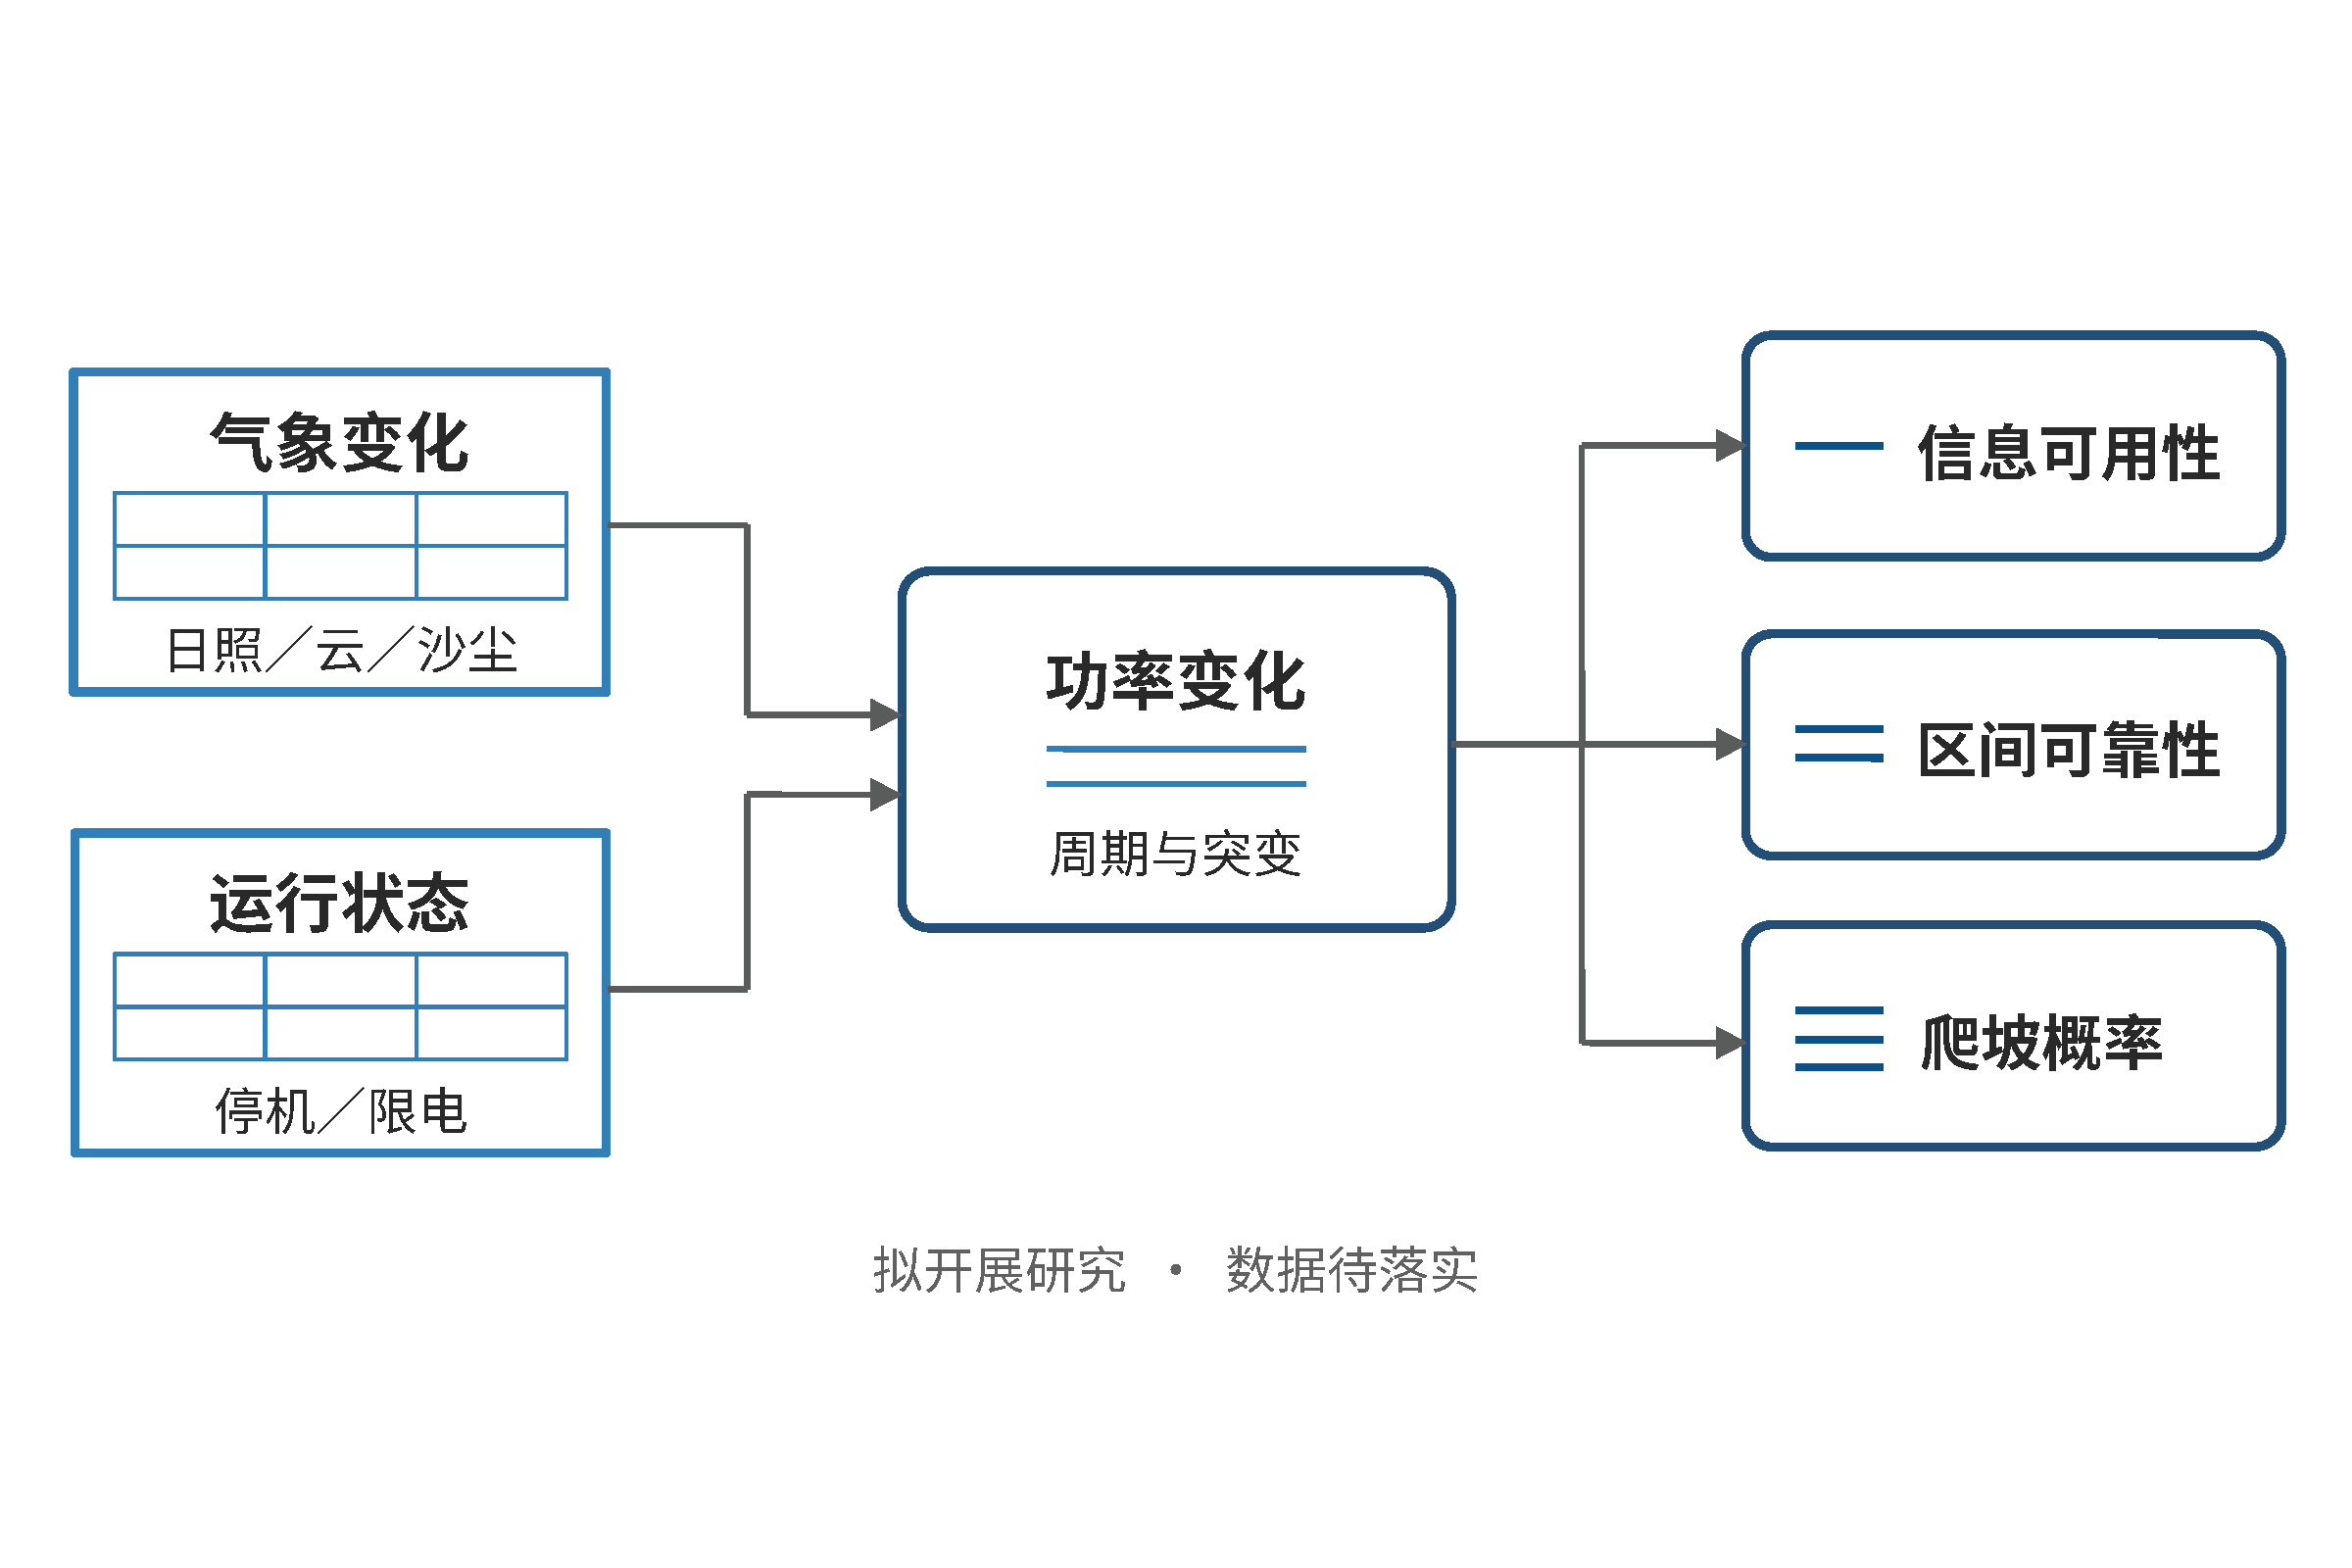
\includegraphics[width=0.94\linewidth]{figures/F01.pdf}
\caption{复杂天气下光伏功率变化与三个待检验问题（拟开展研究，数据待落实）}
\label{fig:xj-f01}
\end{figure}
% NSFC-ILLUSTRATED END F01


\subsubsection{国内外研究现状及发展动态分析}
\textbf{气象驱动与多尺度功率预测。}光伏预测已从历史功率外推发展到气象变量与时序表示的联合建模。Temporal Fusion Transformer研究了多时距预测中的变量选择和时间信息融合\cite{lim2021tft}；DWT-Former利用小波多尺度特征与Transformer时间表示进行光伏预测，WaveKAN进一步探索自适应小波分解与非线性映射结合的长时序建模\cite{sun2025dwt,liu2026wavekan}。FEDformer和TimeMixer分别从频域分解与多尺度混合角度发展时序表示，TimeXer与iTransformer则强化外生信息及变量间关系建模\cite{zhou2022fedformer,wang2024timemixer,wang2024timexer,liu2024itransformer}。这些工作为处理周期与局部波动提供了方法基础，但并不意味着增加模型复杂度必然提升目标场站的预测效果。简单线性方法的系统比较表明，对时序任务仍需保留有竞争力的轻量基线，并控制输入、训练预算和评价方式\cite{zeng2023linear}。

气象变化的尺度结构也已进入概率太阳辐射预报研究。SolarSTEPS按照云变化尺度组织自回归平流预报，深度生成模型则用于延长日内太阳预报时效\cite{carpentieri2023solarsteps,carpentieri2025shadecast}。这类研究提示，空间云运动与时间尺度对预测不确定性都有影响；但辐射场预报与场站电功率预报的对象不同，组件温度、逆变器状态、限电等因素仍需在功率侧处理。现有方法不能直接证明某一尺度或气象变量在新疆所有天气下均有效，本项目需要在相同可用信息条件下，通过去除变量、去除尺度以及跨时间段检验确定增益的边界。

\textbf{概率预测与时序校准。}概率太阳预测已形成明确的基线、后处理和评价框架\cite{gneiting2023solar}。天气场景生成可以把气象不确定性传递到太阳能功率预测，DeepAR等方法则从时间序列直接学习概率预测\cite{sun2020scenario,salinas2020deepar}。相较于仅报告平均绝对误差，适当评分规则同时评价分布的可靠性与集中程度，有助于避免通过无节制扩大区间取得表面覆盖率\cite{gneiting2007proper}。

共形预测为预测区间的校准提供了通用思路，光伏场景已有相应方法和比较研究\cite{renkema2024conformal,solarcp2025comparative}。因此，将共形预测加到光伏模型上本身不能作为本项目的创新。在一般方法层面，共形化分位数回归提供异方差区间构造思路，自适应共形推断（ACI）、集成批量预测区间（EnbPI）和序贯预测共形推断（SPCI）分别处理在线适应、序列残差和条件分数预测；递减步长在线方法进一步讨论更新稳定性\cite{romano2019cqr,gibbs2021aci,xu2021enbpi,xu2023spci,angelopoulos2024online}。时间成分分解与共形预测的结合也已有直接探索\cite{prinzhorn2024decomposition}。需要进一步回答的是，在天气状态改变、误差存在时间依赖且真实标签延迟到达的条件下，校准样本怎样选择，覆盖误差怎样变化，以及改善是否以过宽区间为代价。超出交换性条件的共形预测研究已经说明，覆盖性质受到分布变化和依赖结构制约，不能把独立同分布条件下的结论原样用于任意天气漂移\cite{barber2023beyond}。本项目将区分总体覆盖与天气分组覆盖，以实测检验明确有效范围。

\textbf{从逐时距分布到爬坡事件。}爬坡事件涉及两个及以上时刻的联合变化。即使每个时刻的边际分布完全相同，不同的时间相关结构也会给出不同的功率增量分布。因此，直接相减两个预测区间，或在各时刻独立抽样，不能自动得到可靠的爬坡概率。多变量太阳辐射概率预报基准已将依赖结构纳入评价，变差函数评分等方法也提供了检查多变量预测关系的工具\cite{meer2021benchmark,scheuerer2015variogram}。概率太阳预报用于灵活爬坡产品采购的研究进一步表明，概率输出应面向具体决策对象评价\cite{hobbs2022ramp}，但电力市场采购收益不能直接转写成本项目的场站预警收益。

Schaake shuffle与集合copula耦合已形成“边际后处理后再恢复依赖”的经典思路\cite{clark2004schaake,schefzik2013ecc}。2026年的两项预印本分别关注聚合光伏爬坡的天气关系，以及从未来云演变表征连接功率轨迹与分钟级爬坡预警\cite{lanzilao2026ramp,wang2026skyramp}。它们提示天气与轨迹联合建模仍在发展，但尚不能作为新疆单站方法已成熟有效的证据，也进一步限定了本项目创新应落在具体条件检验上。

上述进展表明，气象融合、多尺度表示、共形校准和概率预警均有明确研究基础。值得继续研究的是它们在同一发布时刻信息约束下如何衔接：天气转换是否改变可利用尺度与残差依赖；后处理改善逐时距区间后，哪些联合结构仍决定事件概率的成败。围绕这一关系开展受控比较，比单纯增加网络模块更能识别本项目的独立贡献。

\subsubsection{现有研究的不足}
第一，气象输入的物理相关性与实际预测可用性经常需要分开判断。未来实况、再分析资料、事后插补以及全序列变换均可能在离线数据处理中进入预测端，使模型使用当时尚不可得的信息。即使回测精度提高，也不足以证明可上线条件下存在同样增益。本项目将以发布和获取时间界定输入，比较真实可用输入与明确标记的理想信息对照，识别气象源、尺度和时距之间的条件关系。

第二，总体覆盖率难以说明复杂天气下区间是否可靠。晴稳时段占多数时，总体指标可能接近目标水平，而天气转换阶段仍系统性漏覆盖。进一步按天气分组又会遇到小样本与状态变化的问题。需要把覆盖偏差、区间评分、样本量及适应延迟一起报告，并通过时间上独立的检验判断改善能否重复出现。对未获支持的条件可靠性，应明确指出其适用限制。

第三，边际概率质量与爬坡事件质量之间仍缺少针对本项目条件的受控验证。若同时替换预测模型、边际分布和轨迹生成方法，事件评价的变化难以归因。本项目将保持各预测时距的样本边际完全一致，只改变跨时距的排序依赖，并与直接预测功率增量的轻量方法比较。这样既能检验时间依赖的作用，也能判断较复杂轨迹方法是否值得采用。

\subsubsection{关键科学问题与研究切入点}
本项目拟回答的中心问题是：\textbf{在预测发布时刻信息受限的条件下，天气变化引起的跨尺度误差及其时间依赖，如何影响光伏概率预测向爬坡事件预警的有效传递？}其中包含三个相互支撑的子问题：气象变量在哪些尺度和时距上提供稳定增益；误差分布变化后滚动校准能否兼顾覆盖与区间效率；边际质量相同时，保留时间依赖能否改善爬坡事件的概率判断。

据此提出可检验的工作假设：在功率与气象数据时间对齐、模型容量和计算预算可比的前提下，天气相关的尺度选择及历史误差校准能够减少部分天气转换时段的预测失配；在相同边际预测下，保留连续误差的秩依赖有望改善爬坡概率的Brier评分，并在固定误报负担下提高事件识别能力。若增益在排除未来信息后消失，校准仅依靠扩大区间改善覆盖，或保留依赖与打散依赖的结果没有稳定差异，则相应假设不获支持。

研究将依次形成可用信息约束的数据与基线、受控的多尺度概率模型、以及可单独检验依赖贡献的爬坡评价。所得结果预期回答哪些输入和结构值得保留、哪些天气条件下方法失效，并据此形成轻量离线预警原型。新疆场站验证的数据与合作落实情况在研究基础部分如实列示，未取得地域实测证据前，不把公开数据实验扩大为新疆应用结论。
